\begin{center}
	\hrule
	\vspace{.4cm}
	{\textbf { \large ELEC 460 --- Control Theory II}}
\end{center}
{\textbf{Name:}\ David Li \hspace{\fill} \textbf{Student Number:}} \ V00818631  \\
{\textbf{Due Date:} Thursday, 11 January 2018, 11:30 AM \hspace{\fill} \textbf{Assignment:} Number 1 \\
	\hrule

    
    
%\tableofcontents
%\newpage


%\subsection*{ELEC 460 Assignment 1}
%%{toc}{subsection}{ELEC 460 Assignment 1}
%\phantomsection
%
%
%\begin{lstlisting}[language = Matlab,frame=single,caption={}]
%clear all
%close all
%\end{lstlisting}


\subsection*{1. Sketch the root locus}
%{toc}{subsection}{1. Sketch the root locus}
\phantomsection


\begin{lstlisting}[language = Matlab,frame=single,caption={}]
G1 = zpk([],[0,-1,-20],20) % create transfer function
figure(1); rlocus(G1) % Plot root locus
\end{lstlisting}

         
% \begin{matlaboutput}{}
%G1 =
% 
%        20
%  --------------
%  s (s+1) (s+20)
% 
%Continuous-time zero/pole/gain model.
%
%\end{matlaboutput}
    
\begin{figure}[h]
	\centering
	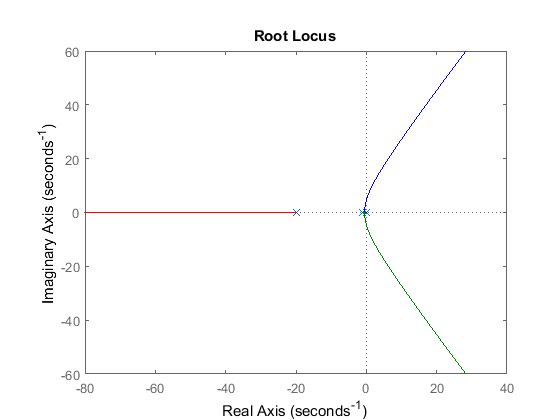
\includegraphics [width=0.7\linewidth]{ELEC460A1_01.png}
	\caption{Root Locus when K =1}
	%\caption{}
	% Alternative is to typeset the caption myself, which makes more sense to me.
	% \label{$fig:ELEC460A1_01.png$}
\end{figure}


\subsection*{2. Find Kv.}
%{toc}{subsection}{2. Find Kv.}
\phantomsection
Using the final value theorem: $x(\infty ) = \mathop {\lim }\limits_{s \to 0} sX(s)$ \newline 

\begin{lstlisting}[language = Matlab,frame=single,caption={}]
syms s ;Kv = limit(s*20/(s*(s+1)*(s+20)),s,0)% compute Kv using limits
\end{lstlisting}


% \begin{matlaboutput}{} 
%Kv =
% 
%1
% 
%\end{matlaboutput}
    

\subsection*{3. Sketch Bode and Nyquist plots.}
%%{toc}{subsection}{3. Sketch Bode and Nyquist plots.}
%\phantomsection


\begin{lstlisting}[language = Matlab,frame=single,caption={}]
figure(2); bode(G1)
figure(3); nyquist(G1)
\end{lstlisting}

\begin{figure}
	\centering
	\begin{minipage}{0.475\textwidth}
		\centering
		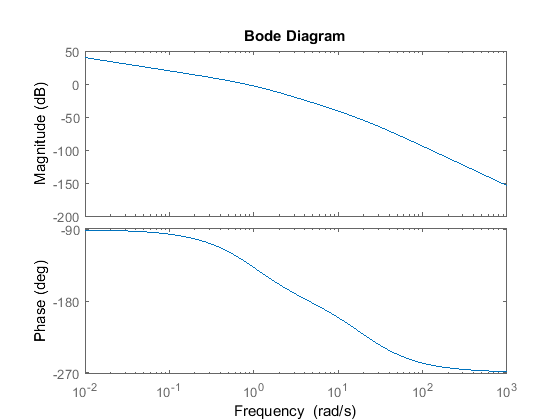
\includegraphics [width=1\linewidth]{ELEC460A1_02.png} % first figure itself
		\caption{Bode plot when K=1}
	\end{minipage}\hfill
	\begin{minipage}{0.475\textwidth}
		\centering
		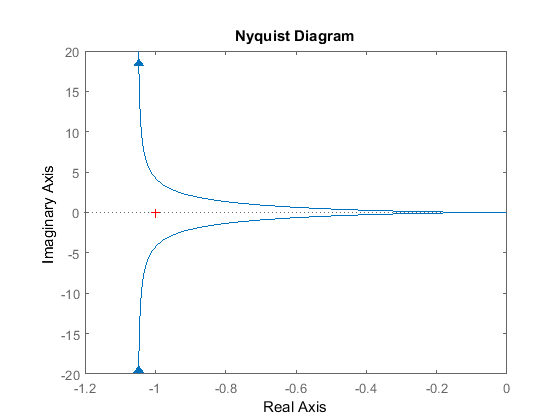
\includegraphics [width=1\linewidth]{ELEC460A1_03.png} % second figure itself
		\caption{Nyquist plot when K=1}
	\end{minipage}
\end{figure}

\subsection*{4. Find K so that $\zeta=\sqrt(2)/2$ for the closed loop system.}
%%{toc}{subsection}{4. Find K so that zeta=sqrt(2)/2 for the closed loop system.}
%\phantomsection

% Consider deleting the zeta value computing and the fprintf
%\begin{lstlisting}[language = Matlab,frame=single,caption={}]
%zeta = sqrt(2)/2
%figure(4);
%gains = -1:0.00125:1;
%rlocus(G1,gains); sgrid; K = 0.476;
%% Plot test box with results onto plot
%gainString = ['Gain: ' num2str(K)];text(-0.25,0.5,gainString);
%fprintf('Using the root locus the value K at which zeta is 0.7071 is: %0.3f. \n', K )
%\end{lstlisting}

% Rewrite using latex commands   
% \begin{matlaboutput}{}
%zeta =
%
%    0.7071
%
%Using the root locus the value K at which zeta is 0.7071 is: 0.476. 
%\end{matlaboutput}
    % I think I might remove this picture
Using the root locus the value K at which $\zeta$ is 0.7071 is: 0.476. 
%\begin{figure}[h]
%	\centering
%	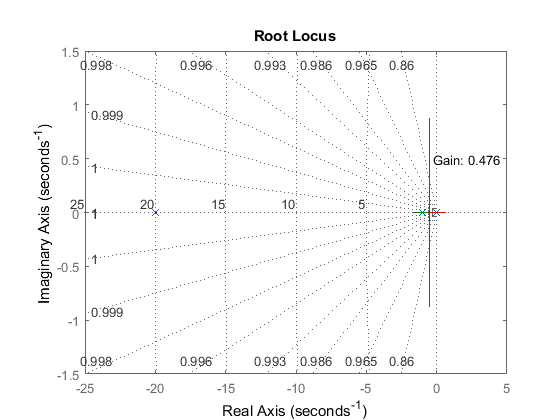
\includegraphics [width=0.7\linewidth]{ELEC460A1_04.png}
%	\caption{$ELEC460A1_04.png$}
%	%\caption{}
%	% Alternative is to typeset the caption myself, which makes more sense to me.
%	% \label{$fig:ELEC460A1_04.png$}
%\end{figure}


\subsection*{5. Find phase and gain margins for this K.}
%%{toc}{subsection}{5. Find phase and gain margins for this K.}
%\phantomsection


\begin{lstlisting}[language = Matlab,frame=single,caption={}]
G1new = zpk([],[0,-1,-20],20*K)
figure(5); margin(G1new)
\end{lstlisting}
    
\begin{figure}[ht]
	\centering
	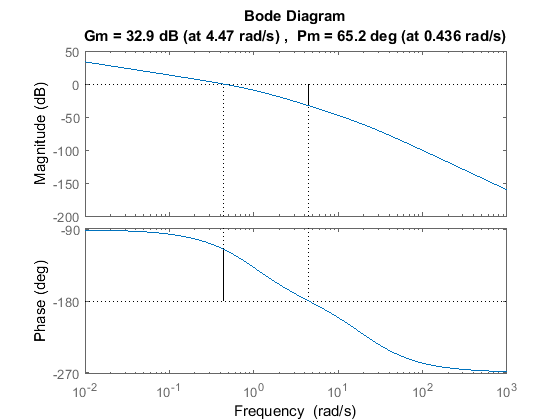
\includegraphics [width=0.7\linewidth]{ELEC460A1_05.png}
	\caption{Phase and Gain Margin in Bode Plot}
	%\caption{}
	% Alternative is to typeset the caption myself, which makes more sense to me.
	% \label{$fig:ELEC460A1_05.png$}
\end{figure}


\subsection*{6. Sketch the step and ramp responses of the closed loop system for this K}
%%{toc}{subsection}{6. Sketch the step and ramp responces of the closed loop system for this K}
%\phantomsection


\begin{lstlisting}[language = Matlab,frame=single,caption={}]
G1tfnew = tf(G1new)
subplot(2,1,1); step(G1tfnew); %% create subplot for step function
ramps = tf([1,0],[1]);
subplot(2,1,2); step(G1tfnew/ramps); %% create subplot for ramp function
\end{lstlisting}

         
% \begin{matlaboutput}{}
%G1tfnew =
% 
%         9.52
%  -------------------
%  s^3 + 21 s^2 + 20 s
% 
%Continuous-time transfer function.
%
%\end{matlaboutput}
    
\begin{figure}[ht]
	\centering
	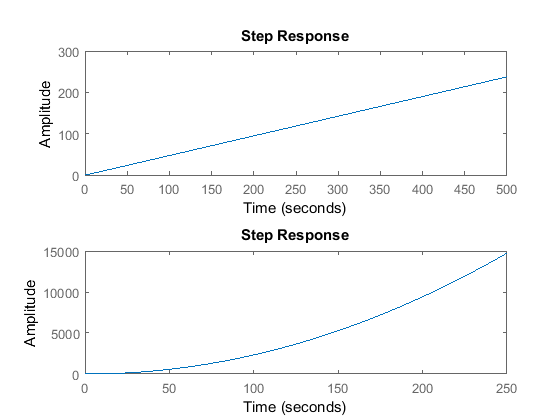
\includegraphics [width=0.7\linewidth]{ELEC460A1_06.png}
	\caption{Step Response of Transfer function with K = 0.479}
	%\caption{}
	% Alternative is to typeset the caption myself, which makes more sense to me.
	% \label{$fig:ELEC460A1_06.png$}
\end{figure}


\subsection*{7. Discuss the connection between Kv, zeta, margins and the response of the closed loop system.}
%{toc}{subsection}{7. Discuss the connection between Kv, zeta, margins and the response of the closed loop system.}



   The value of Kv is 1, so the steady state velocity error is constant. Additionally 
   the system is stable because of a positive phase and gain margin. Finally, the value of 
  $\zeta = 0.7071$ corresponds to a gain of 0.427.   \newline